%!TEX root = ../cwqo.tex
\section{Bad Patterns In Tree Decompositions}
\label{sec:bad-patterns}

We will make heavy usage of the results of \cite{COLC07} on trees.

\todo[inline]{First, we restrict ourselves to simple interpretations, i.e.,
    those that are defined solely by a formula $\varphi_E(x,y)$ defining
the edge relation}

\subsection{From Interpretation to Monoids}

\AP We use unranked ordered trees $T$ with labels taken from a finite alphabet
$\Sigma$ placed on the nodes of the trees. These trees are denoted using
$\Trees{\Sigma}$. In a tree, the root is denoted by $\treeRoot$, and the set of
leaves is denoted by $\Leaves{T}$. Given two nodes $x$ and $y$ in a tree $T$,
their least common ancestor is denoted by $\lca(x,y)$. Given two nodes $x,y$
such that $y$ is an ancestor of $x$, the notation $T[x:y]$ denotes the
\emph{word} in $\Sigma^*$ obtained by reading the labels of the nodes on the
path from $x$ to $y$ in $T$. 


\begin{lemma}
    \label{interpretation-to-monoid:lem}
    Let $\Sigma$ be a finite alphabet, and $I$ be an $\MSO$ interpretation
    from $\Trees{\Sigma}$ to $\Graphs$.
    There exists a finite monoid $M$, a morphism
    $\mu \colon \Sigma \to M$,
    and a subset $P \subseteq M^3$ such that
    \begin{align*}
        &\forall T \in \Trees{\Sigma},
        \forall x,y \in \Leaves{T}, \\
        &\varphi(x,y) = \top \\
        &\iff \\
        &(\mu(T[\lca(x,y) \colon x]), 
          \mu(T[\treeRoot \colon \lca(x,y)]), 
          \mu(T[\lca(x,y) \colon y])) \in P
    \end{align*}
\end{lemma}

\begin{figure}
    \centering
    \begin{tikzpicture}[
        leaf/.style={
            color=Prune
        },
        lca/.style={
            color=A1
        },
        edge/.style={
            color=A2
        },
        root/.style={
            color=Prune
        },
        gedge/.style={
            color=A4
        },
        ]
        \node[root] (root) at (0,1) {$\treeRoot$};
        \node[leaf] (x) at (-1,-1) {$x$};
        \node[leaf] (y) at (1,-1) {$y$};
        \node[lca] (lca) at (0,0) {$\lca(x,y)$};
        \coordinate (tl) at ($(x.south west)+(-0.2,0)$);
        \coordinate (tr) at ($(y.south east)+(0.2,0) $);
        \coordinate (t)  at ($(root.north)+(0, 1)$);
        \draw[edge,->] (root) to node[midway, left]        {$a$}  (lca);
        \draw[edge,->] (lca)  to node[midway, above  left] {$b$} (x);
        \draw[edge,->] (lca)  to node[midway, above right] {$c$} (y);
        \draw (tl) -- (tr) -- (t) -- cycle;

        \node (maps-to) at (3,0) {$\mapsto$};

        \begin{scope}[xshift=4cm]
            \node[leaf] (nx) at (0,0) {$x$};
            \node[leaf] (ny) at (5,0) {$y$};
            \draw[gedge] (nx) to node[midway, above] {$(a,b,c) \in P$?} (ny);
        \end{scope}
    \end{tikzpicture}
    \caption{The interpretation of a tree using a monoid and an accepting part.}
    \label{interpretation-to-monoid:fig}
\end{figure}

\AP This combinatorial description of the interpretation in terms of a monoid
allows us to introduce the notion of \emph{edge labelled tree}. We use the
notation $\Trees[M]{\Sigma}$ for the trees where the vertices are labelled by
elements of $\Sigma$ and the edges are labelled by elements of $M$. To simplify
notations, we will allow ourselves to write $\mu[T](x,y)$ for $\mu(T[x \colon
y])$ and omit $T$ when it is clear from the context.


It is quite clear how one interprets a graph using such a tree and a subset $P
\subseteq M^3$. One simply takes as vertices the leaves of the tree, and adds
an edge between two vertices $x$ and $y$ if the ``triangle condition'' is
satisfied. 

\todo[inline]{Explain how the new tree interpretation works, using 
    the so-called \emph{composition ordering} on trees labelled by
    a finite monoid}

\AP
\begin{definition}
    \label{composition-ordering:def}
    Let $T$ and $T'$ be two trees in $\Trees[M]{\Sigma}$. We say that $T \cmpleq T'$
    if there exists a map $h \colon T \to T'$ such that
    for any pair $x \leq_T y$ of nodes in $T$,
    we have $h(x) \leq_{T'} h(y)$ and
    $\mu(x,y) = \mu(h(x), h(y))$.
\end{definition}



\begin{figure}
    \centering
    \todo[inline]{Draw the composition ordering on trees}
    \caption{The composition ordering on trees}
    \label{composition-ordering:fig}
\end{figure}

\subsection{Forward Ramseyan Splits and Bad Branches}

\todo[inline]{Recall that in the case of words, there exists a factorisation theorem
    due to Simon, explain that this will be an equivalent for trees.}

\def\t{\aTree}

\AP Let $\t$ be a finite tree with edges labelled by elements of a finite
monoid $M$. We write $\tlbl{\t}{x}{y}$ whenever $x \treelt[\t] y$ for the
product of the edge labels on the path from $x$ to $y$ in $\t$.

A \intro{split of height $N$} of $\t$ is a mapping $\spt$ from the
nodes of $T$ to $\set{1, \dots, N}$. Given a split $\spt$, two elements $x
\treelt[\t] y$ such that $\spt(x) = \spt(y) = k$ are \intro{$k$-neighbours} if
$\spt(z) \geq k$ for all $z$ in the \kl(tree){path} from $x$ to $y$ in $\t$. A
split $\spt$ is \intro{forward Ramseyan} if for every $k \in \set{1, \dots, N}$ and
every $x, y, x', y'$ in the same class of $k$-neighbourhood with $x \treelt[\t] y$
and $x' \treelt[\t] y'$, we have 
\begin{equation} 
    \label{fake-idempotent:eq}
    \tlbl{\t}{x}{y} = \tlbl{\t}{x}{y} \cdot \tlbl{\t}{x'}{y'} \quad ,
\end{equation}
In particular, $\tlbl{\t}{x}{y}$ is an \kl{idempotent},
but $\tlbl{\t}{x}{y}$ and $\tlbl{\t}{x'}{y'}$ may be different \kl{idempotents}.

\AP Let us illustrate how one can use \kl{forward Ramseyan splits} to compute
efficiently the value of $\tlbl{\t}{x}{y}$ for any pair of nodes $x \treelt[\t]
y$. We are going to paraphrase the actual content of \cite[Lemma 3]{COLC07},
using the drawing of \cref{fast-computation:fig}
to
explain the idea. Given two nodes $x \treelt[\t] y$ in a tree $\t$, let us
define $\spt(x:y)$ to be the minimal value of $\spt(z)$ for $x \treelt[\t] z
\treelt[\t] y$, and $N+1$ if there is no such $z$. We claim that to compute the
value of $\tlbl{\t}{x}{y}$, one can restrict the computation to specific
segments of the path with a \emph{strictly larger} value of $\spt$. The reason
is that whenever $x$ and $y$ are separated by many nodes $z$ such that $\spt(z)
= \spt(x:y)$, one can essentially ignore all but the first and last such nodes
to speed up computation. This of course can be applied recursively leading to a
fast (and first-order definable, provided the split $\spt$ is known) algorithm
to compute the value of $\tlbl{\t}{x}{y}$.

\begin{figure}
    \centering
    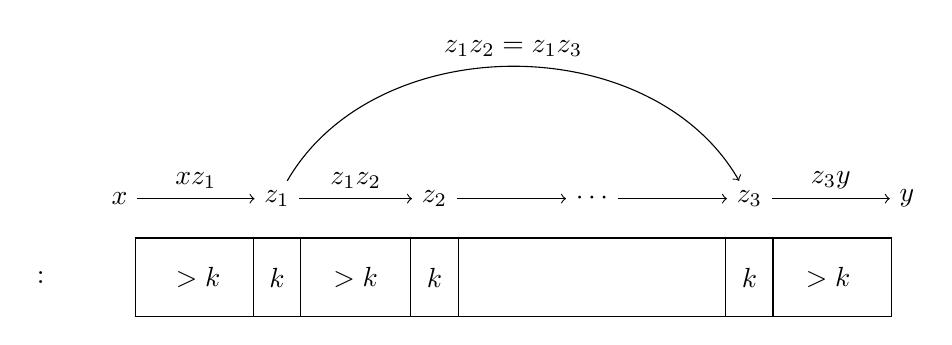
\begin{tikzpicture}
        \node (s) at (-1,-1) {$\spt \colon $};
        \node (x) at (0,0) {$x$};
        \node (z1) at (2,0) {$z_1$};
        \node (z2) at (4,0) {$z_2$};
        \node (z3) at (6,0) {$\cdots$};
        \node (z4) at (8,0) {$z_3$};
        \node (y) at (10,0) {$y$};

        \node[below of=z1] {$k$};
        \node[below of=z2] {$k$};
        \node[below of=z4] {$k$};
        \node (xz1) at (1,-1) {$> k$};
        \node (z1z2) at (3,-1) {$> k$};
        \node (z4y) at (9,-1) {$> k$};

        \draw (0.2,-0.5) rectangle (9.8,-1.5);
        \draw (1.7,-0.5) -- (1.7, -1.5);
        \draw (2.3,-0.5) -- (2.3, -1.5);

        \draw (3.7,-0.5) -- (3.7, -1.5);
        \draw (4.3,-0.5) -- (4.3, -1.5);

        \draw (7.7,-0.5) -- (7.7, -1.5);
        \draw (8.3,-0.5) -- (8.3, -1.5);


        \draw[->] (x) -- 
        node[midway, above] {$\tlbl{\t}{x}{z_1}$}
        (z1);
        \draw[->] (z1) --
        node[midway, above] {$\tlbl{\t}{z_1}{z_2}$}
        (z2);
        \draw[->] (z2) -- (z3);
        \draw[->] (z3) -- (z4);
        \draw[->] (z4) -- 
        node[midway, above] {$\tlbl{\t}{z_3}{y}$}
        (y);
        \draw[->] (z1) to[bend left=60] 
        node[midway, above] {$\tlbl{\t}{z_1}{z_2} = \tlbl{\t}{z_1}{z_3}$}
        (z4);

    \end{tikzpicture}
    \caption{Fast computation of the value $\tlbl{\t}{x}{y}$
        provided a forward Ramseyan split.}
    \label{fast-computation:fig}
\end{figure}


\AP This idea can be refined to understand the behavior of leaves in the tree
with respect to a given branch. This is the motivation for the following
definition of \kl{boughs}, which are specific slices of a branch the tree.

\begin{definition}
    \label{ramseyan-branch:def}
    Let $T$ be a tree and $\spt$ be a \kl{forward Ramseyan split} of height $N$.
    A \intro{bough of level $k$} in $T$ is an infix of a branch of $T$
    satisfying:
    \begin{enumerate}
        \item Its maximal and minimal elements have level $k$
        \item All elements of the bough have level greater or equal to $k$
    \end{enumerate}
    The \intro{size of a bough} is the number of elements of depth $k$
    in the \kl{bough}.
\end{definition}

\AP Let $B$ be a \kl{bough of level $k$} in $T$. Given two nodes $b_1$ and
$b_2$ in $B$ such that $\spt(b_1) = \spt(b_2) = k$, we define the $T_{b_1:b_2}$
as the set of nodes $x$ in $T$ such that $b_1 \treeleq x$ and $\neg (b_2
\treeleq x)$. For every leaf $x \in T_{b_0: b_n}$ where $n$ is the size of the
bough $B$, we define $\Bt(x)$ to be the least ancestor of $x$ that belongs to
$B$. Similarly, we define $\Bl(x)$ to be the least element of $B$ that is
greater or equal to $\Bt(x)$, and $\Br(x)$ to be the greatest element of $B$
that is less or equal to $\Bt(x)$. To every leaf $x$ of $B(T)$, we can
therefore associate a triple of values: $\BtL(x) \defined
\tlbl{\t}{\Bt(x)}{x}$, $\BlL(x) \defined \tlbl{\t}{\Bl(x)}{\Bt(x)}$, and
$\BrL(x) \defined \tlbl{\t}{\Bt(x)}{\Br(x)}$. We refer to
\cref{type-of-a-leaf-in-branch:fig} for an
illustration of the type of a leaf with respect to a given \kl{bough} $B$.
We also refer to \cref{partitionning-a-graph:fig} for an illustration of the
resulting partition of the tree $T$ with respect to a given \kl{bough} $B$.

\begin{figure}
    \centering
    \begin{tikzpicture}[
        branch/.style={
            color=Prune,
            inner sep=0pt,
            minimum size=4pt,
            fill,
            circle
        },
        inner/.style={
            color=A1,
            inner sep=0pt,
            minimum size=4pt,
            draw,
            circle
        },
        staredge/.style={
            color=A1,
            ->,
            dashed
        },
        root/.style={
            color=Prune,
        },
        leaf/.style={
            color=Prune,
        },
        monoid/.style={
            color=A2
        },
        ]
        % first draw the branch 
        \node[root]   (root) at (-2,0) {$\treeRoot$};
        \node[branch] (b0) at (0,0) {};
        \node[branch] (b1) at (4,0) {};
        \node[inner]  (t)  at (2,0) {};
        \node[leaf]   (x)  at (3.5,-2) {$x$};

        \node[above=0.1cm of b0] {$\Bl(x)$};
        \node[above=0.1cm of t]  {$\Bt(x)$};
        \node[above=0.1cm of b1] {$\Br(x)$};

        \draw[staredge] (root) -- (b0);
        \draw[staredge] (b0) -- node[monoid, midway, below] {$\BlL(x)$} (t);
        \draw[staredge] (t)  -- node[monoid, midway, below] {$\BrL(x)$} (b1);
        \draw[staredge] (b1) -- (5,0);

        \draw[staredge] (t)  -- node[monoid, midway, below left] {$\BtL(x)$} (x);
    \end{tikzpicture}
    \caption{The type of a leaf with respect to a given \kl{bough} $B$.}
    \label{type-of-a-leaf-in-branch:fig}
\end{figure}

\begin{figure}
    \centering
    \begin{tikzpicture}[
        localType/.style={
            color=C3,
            thick
        },
        branchProj/.style = {
            color=Prune,
            inner sep=0pt,
            minimum size=4pt,
            fill,
            circle
        },
        leaf/.style={
            color=Prune,
        },
        ]
        \draw (0,0) rectangle (8,2);
        \node (root) at (-2,2) {$\treeRoot$};
        \foreach \x in {0,1,2,3,4} {
            \coordinate (n\x) at ({ 2 * \x},0);
            \coordinate (pb\x) at ({ 2 * \x},2);
            \node[branchProj] (b\x) at (pb\x) {};
            \node (lb\x) at ({ 2 * \x},2.4) {$b_{\x}$};
            \draw (n\x) -- (b\x);
        }
        \draw[dashed,<-] (b0) -- (root);
        \draw[dashed] (b4) -- (9,2);
        \draw[dashed] (n4) -- (9,0);

        \foreach[count=\x] \y in {0,1,2,3} {
            \node (E\x) at ({ 2 * \x - 1},2.6) {$e_{\y}$};
            \draw[->,thick] (b\y) to[bend left=40] (b\x);
            \node (T\x) at ({ 2 * \x - 1},-0.6) {$T_{b_{\y}:b_{\x}}$};
        }
        
        \node (x) at (3,0.2)  {$x$};
        \node (y) at (7,0.2)  {$y$};
        \node[branchProj] (tx) at (3,2) {};
        \node[branchProj] (ty) at (7,2) {};

        \draw[localType, <-] (x)  -- 
        node[midway, left] {$\BtL(x)$} (tx);
        (tx);
        \draw[localType, ->] (tx) -- 
        node[midway, below] {$\BrL(x)$}
        (b2);
        \draw[localType, <-] (tx) -- 
        node[midway, below] {$\BlL(x)$}
        (b1);

        \draw[localType, <-] (y)  -- 
        node[midway, left] {$\BtL(y)$} 
        (ty);
        \draw[localType, ->] (ty) -- 
        node[midway, below] {$\BrL(y)$}
        (b4);
        \draw[localType, <-] (ty) --
        node[midway, below] {$\BlL(y)$}
        (b3);


    \end{tikzpicture}
    \caption{Partitionning a graph using a branch.}
    \label{partitionning-a-graph:fig}
\end{figure}

\AP
To compute the presence of an edge between two leaves $x$ and $y$
in $B(T)$, we only need to know their respective \kl{bough types}
the order in which they appear in the \kl{bough}, 
and whether or not there is an idempotent. \cref{partitionning-a-graph:fig}.

\begin{definition}
    \label{good-bough:def}
    Let $T$ be an edge-$M$-labelled tree, $\spt$ be a \kl{forward Ramseyan split}
    of height $N$, and $B$ be a \kl{bough} of level $k$ in $T$.
    The \kl{bough $B$} is a \intro{good bough} if, for every element $m \in M$,
    there exists a branch $H$ of depth $k$ in some other tree $T'$ in $\Trees[M]{\Sigma}$
    and a function $h \colon B(T) \to H(T')$ such that
    \begin{itemize}
        \item The subgraph generated by $m B(T)$ embeds into the subgraph generated by $m H(T')$ via $h$.
        \item The image of the root of $B$ by $h$ is the root of $H$.
        \item The image of the last element of $B$ by $h$ the last element of $H$.
        \item The map $h$ respects the $3$-types of the leaves.
    \end{itemize}
\end{definition}

\begin{lemma}
    Assume that there are no bounds on the $k$-length of bad branches, then 
    the class of images is not $(3 \times \card{M}^3)$-well-quasi-ordered.
\end{lemma}
\begin{proof}
    Let $\seqof{B_i}$ be an infinite sequence of bad branches of strictly increasing $k$-length.
    This means that for every $i$ there exists an $m_i \in M$ such that
    no branch $H$ can contain $m B_i(T)$. By extracting a subsequence, we can assume that $m$ is constant.
    Extracting more, we can assume that the $k$-length of $B_i$ is greater than three times the
    number of nodes in $B_{i-1}$.

    Look at the generated graphs, colored by the $3$-types of the leaves plus
    distinguishing colors for the root and last elements of the branches. Assume by contradiction that
    there exists an embedding from $T_i$ to $T_j$ for some $i < j$. Then,
    this is also an embedding between $B_i(T_i)$ and $B_i(T_j)$, and
    shows that $B_i(T_i)$ is a \kl{good branch} which is a contradiction.
\end{proof}

\begin{lemma}
    One can decide whether there exists unbounded
    bad branches.
\end{lemma}
\begin{proof}
    We consider the automaton that reads from a decorated tree
    the bough $B$, the partition, the type of the leaves. 
    It first checks that the decoration is correct, and then
    guesses whether the decoration would still be good when
    mapping every leaf of the bough to either a "left" or a "right"
    duplicate of this branch. This is an $\MSO$-definable property.
    It suffices to check that the corresponding automaton
    has an unbounded language, which is decidable.
\end{proof}

\subsection{Good Expansion of A Tree}

The idea now is to use the uniform bound on bad branches to construct an
\emph{expanded} version of any tree, allowing us to correctly use gap
embeddings.

\begin{lemma}
    Let $T$ be a tree and let $B$ be a good branch. Then, one can embed     
    $B$ into three copies of itself.
\end{lemma}
\begin{proof}
    TODO. Be careful about idempotents but it should be ok.
\end{proof}

\begin{definition}
    The \intro{generalized gap embedding relation}
    between trees.
    between two trees and a dependency relation $\Delta$
    is ...
\end{definition}

\begin{lemma}
    If $T$ embeds into $T'$ via the \kl{generalized gap embedding relation}
    then their \kl{marked subgraphs} embed into each other.
\end{lemma}
\begin{proof}
    To prove that, consider $x,y$ two leaves
    in $T$, and their least common ancestor $z$.
    We want to prove that
    $\tlbl{\t}{z}{x} = \tlbl{\t'}{h(z)}{h(x)}$.
\end{proof}

\begin{lemma}
    Assume that there is a bound $N_0$ on the length of bad branches, then
    one can embed any tree $T$ into a tree $T'$ with a ramseyan split of height $XXX$
    with a dependency relation of length at most $XXX$.
\end{lemma}
\begin{proof}
    This is done by grouping the $k$-neighbours of the tree $T$ into buckets of length $N_0 + 1$, and then
    splitting those buckets. 
\end{proof}

The proof of the following theorem is now straightforward, provided that one
knows that the \kl{generalized gap embedding relation} is a
well-quasi-ordering. This is not true in general
(\cref{bad-generalized-gap:ex}), but it will be true when the
dependency relation is bounded (\cref{good-generalized-gap:thm}).
Note that this is not a direct consequence of the classical result of
\cite{DERSHOWITZ200380}, precisely because of the presence of the dependency
relation. At a high level though, this is the same idea.

\begin{example}
    \label{bad-generalized-gap:ex}
    todo
\end{example}


\begin{proofof}{effective-image:thm}[main]
    Test
\end{proofof}

\begin{corollary}
    \label{effective-image:cor}
    A class of graphs $\Cls$ of \kl{bounded clique width} 
    is \kl{labelled-well-quasi-ordered}
    if and only if it is \kl{wqo-well-quasi-ordered}.
\end{corollary}
\begin{proof}
    Consider a class $\Cls$ of graphs having bounded clique width.
    There is an interpretation from trees to a superset of this class $\Cls$.
    Because $\Cls$ is \kl{labelled-well-quasi-ordered}, the class of images
    can be described using finitely many forbidden patterns,
    and we can assume that we do not take subsets.
    Furthermore, we can also encode the node selection into the edges.
    As a consequence, we can assume that there exists a $\varphi$
    such that $\Cls \subseteq \varphi(\Trees{\Sigma}) \subseteq \dwset{\Cls}$.
    Now, because $\Cls$ is \kl{labelled-well-quasi-ordered}, we can assume that
    $\dwset{\Cls}$ is \kl{labelled-well-quasi-ordered} as well.
    This proves that $\varphi(\Trees{\Sigma})$ is \kl{labelled-well-quasi-ordered},
    hence \kl{wqo-well-quasi-ordered},
    and as a consequence so is $\Cls$.
\end{proof}

\section{Neighbour Respecting Gap-Embedding}
\label{sec:neighbour-respecting-gap-embedding}

The goal of this subsection is to prove that the gap-embedding relation with a
bounded dependency relation is well-quasi-ordered. Unfortunately, encoding the
dependency inside the usual notion of gap-embedding (the one without
dependencies) is non-trivial. We will instead leverage the recent advances in
inductively defined well-quasi-orderings \cite{FREU20,LOPEZ23}, and the
characterization of the gap-embedding relation as an inductive Kruskal
construction \cite{FREU20} to conclude.

\begin{equation*}
    T_{k+1}^N (X) \defined
    \mu Y. T_{k}^N( \cdots T_k^N(Y) \cdots ) + X
\end{equation*}

And then we use \cite{LOPEZ23} to conclude that it is a WQO + induction 
to prove that it respects the "first-$N$-neighbours".
\begin{theorem}
    \label{good-generalized-gap:thm}
    The gap ordering associated to the ramseyan split of height $XXX$ is a well-quasi-ordering.
\end{theorem}
\begin{proof}
    Trivial. \todo{Not at all!!}
\end{proof}

TODOs:
\begin{itemize}
    \item Define the simon's factorisation theorem for trees.
    \item Check that we can assume that "all products are nice" and not just the ones
        appearing in the decomposition.
    \item Define "branch decompositions" and the "type of nodes" in a branch decomposition.
    \item Define a "bad branch"
    \item Prove that arbitrarily large bad branches violate WQO.
    \item Prove that "good branches" can be embedded into three copies of themselves
    \item Define the "good expansion" of a tree $T$ by expanding all good branches.
    \item Update the tree-decomposition of this good expansion to add \emph{non-sibling}
        idempotent nodes.
    \item Prove that the good expansions of a tree $T$ are well-quasi-ordered using a 
        suitable gap embedding.
    \item Conclude that the class of images is WQO.
\end{itemize}

\begin{lemma}
    \label{gap-embedding-ramseyan:lem}
    Let $(\t, \spt)$ be a tree with a forward Ramseyan split of height $N$,
    and $(\t', \spt')$ be another tree with a forward Ramseyan split of height $N$.
    Let $h \colon \t \to \t'$ be a map such that for every $x,y \in \t$
    we have 
    \begin{itemize}
        \item $h$ maps leaves to leaves. (respects the tree shape)
        \item $h(\lca(x,y)) = \lca(h(x), h(y))$  (respects the tree shape)
        \item $h(\spt(x)) = \spt'(h(x))$ (locally respects splits)
        \item on every branch, for every node $x$ that has a successor 
            $\tlbl{\t}{x}{x+1} = \tlbl{\t'}{h(x)}{h(x)+1}$ (locally respects edges)
        \item $\min\setof{ \spt(z) }{x \treeleq[\t] z \treeleq[\t] y} = \min\setof{ \spt'(z) }{h(x) \treeleq[\t'] z \treeleq[\t'] h(y)}$
            (globally respects nestings)
    \end{itemize}
    Then the embedding $h$ satisfies for all $x,y$ such that
    there exists $x \treeleq[\t] z_1 \treelt[\t] z_2 \treeleq[\t] y$, 
    with $\spt(z_1) = \spt(z_2) = \min\setof{\spt(z)}{x \treeleq[\t] z \treeleq[\t] y}$, we have
    \begin{equation*}
        \tlbl{\t}{x}{y} = \tlbl{\t'}{h(x)}{h(y)} \quad .
    \end{equation*}
\end{lemma}
\begin{proof}
    We prove this by induction on $k = \min\setof{\spt(z)}{x \treeleq[\t] z \treeleq[\t] y}$.
    The base case is when $k = N$.
    In this case, every node on the path from $x$ to $y$ has \kl{split value} $N$.
    In particular, $\tlbl{\t}{x}{y} = \tlbl{\t}{x}{x+1}$. Now, because $h$ locally 
    respects the edges, we have $\tlbl{\t'}{h(x)}{h(x)+1} = \tlbl{\t'}{h(x)}{h(y)}$,
    and we are done.

    Now, assume that the property holds for $k+1$. Let $x,y$ be such that there
    exists $x \treeleq[\t] z_1 \treelt[\t] z_2 \treeleq[\t] y$ with $\spt(z_1)
    = \spt(z_2) = k$. Let us write $z_3$ for the last node on the path from
    $z_2$ to $y$ such that $\spt(z_3) = k$, and assume that between $x$ and
    $z_1$ there is no node with split value $k$, similarly between $z_1$ and
    $z_2$ and  $z_3$ and $y$.

    By induction hypothesis, we know that $\tlbl{\t}{x}{z_1} =
    \tlbl{\t'}{h(z_2)}{h(z_3)}$. Now, we

\end{proof}
